\section{Проектирование системы}
\label{sec:Chapter3} \index{Chapter3}
\subsection{Функции, предоставляемые библиотекой}

Для выполнения различных сценариев работы с документами и требованиями библиотека должна предоставлять следующие функции:

\begin{itemize}
\item \textbf{Получение объектной модели документа}

Согласно \cite{book:DOM}, \cite{book:JDOM}, \textbf{Объектная модель документа} (Document Object Model – DOM) – стандарт, предложенный веб-консорциумом, и регламентирующий способ представления содержимого документа (в частности – xhtml документа) в виде набора объектов. DOM позволяет представить любой документ в виде иерархической структуры (дерева) узлов, каждый из которых соответствует элементу, атрибуту, текстовому, графическому или любому другому объекту.

Одним из инструментов, позволяющих извлекать DOM модель документа из текстового файла, является библиотека JDOM (в данной работе используется версия 2.0.6).

По документу осуществляется получение структуры данных (дерева), соответствующего объектной модели документа. Схематичный пример полученного из документа DOM дерева изображен на рисунке \ref{pr:image4}.

\begin{figure}[h]
\begin{center}
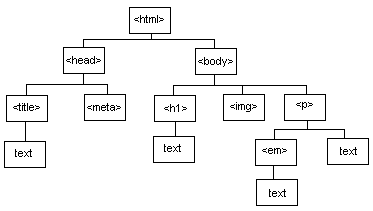
\includegraphics[scale=1.4]{dom.png}
\caption{\emph{Пример DOM модели документа}}
\label{pr:image4}
\end{center}
\end{figure}

\item \textbf{Выделение структурной разметки документа из его DOM дерева}

По DOM модели документа осуществляется построение дерева, отражающего его структурную разметку.

\item \textbf{Получение списка требований по дереву документа}

Выделение фрагментов требований из дерева с дальнейшей группировкой по id. 

Из дерева структурной разметки документа извлекается список требований(объектов), каждое требование содержит идентификационный номер и список фрагментов текста, содержащихся в нем.

\item \textbf{Синхронизация по фрагменту требования}

По фрагменту требования находится вершина дерева разметки исходного документа, в тексте раздела которой содержится данный фрагмент.

\item \textbf{Получение пути в дереве разметки от корня до элемента}

По дереву разметки документа осуществляется поиск последовательности вершин – пути в дереве от корня до данной вершины.

\item \textbf{Поиск элемента, соответствующего данному, в дереве другого документа}

По элементу дерева разметки одного документа осуществляется поиск элемента разметки другого документа такого, что пути из корней деревьев до элементов имеют одинаковые типы вершин и идентичный (с точностью до незначащих символов) текст соответствующих заголовков.

\item \textbf{Перенос объединения фрагментов требования}

В конечном документе осуществляется поиск участка текста, соответствующего объединению фрагментов требования, и осуществляется перенос тегов фрагментов в найденные позиции (начало и конец найденного участка текста).

\item \textbf{Перенос требования}

Попытка переноса всех фрагментов требования.

\end{itemize}

\subsection{Использование библиотеки JDOM}

Важным этапом работы любого алгоритма, решающего поставленную задачу, является получение и хранение содержимого исходного и конечного документов. Одним из инструментов, позволяющих это сделать, является библиотека JDOM, используя которую можно получить DOM модель по XML документу. Также JDOM позволяет эффективно получить все фрагменты требований из исходного документа.

Помимо этого, JDOM предоставляет средства для редактирования XML документов, что является лучшим способом добавить разметку в конечную версию документа после осуществления переноса  фрагментов требований.

В статье \cite{web:JDOM} описываются возможности и приводятся примеры использования JDOM.

\subsection{Обзор решения, применяемого в Requality}

\subsubsection{Основная идея}

Решение проблемы переноса разметки требований, использующееся на данный момент в Requality, основано на сравнении исходного и конечного документа без XHTML разметки, как строк текста (plain text). Для сравнения используется библиотека google-diff, в качестве результата сравнения двух текстов возвращающая список объектов Diff, каждый из которых содержит описание операции, которую нужно выполнить с текстом исходного документа.

Статья \cite{web:Diff} описывает ключевой алгоритм, использующийся в google-diff.

Операции имеют формат \emph{(<Тип операции>, <Текст>)}, где \emph{Тип операции} - одна из трех команд "EQUAL"\, "DELETE"\, "INSERT"\, а \emph{Текст} - часть текста исходного документа, над которой операцию необходимо совершить. Гарантируется, что при последовательном выполнении операций из списка из текста исходного документа получится текст конечного. Пример результата работы Diff алгоритма изображен на рисунке \ref{pr:image5}.

\begin{figure}[h]
\begin{center}
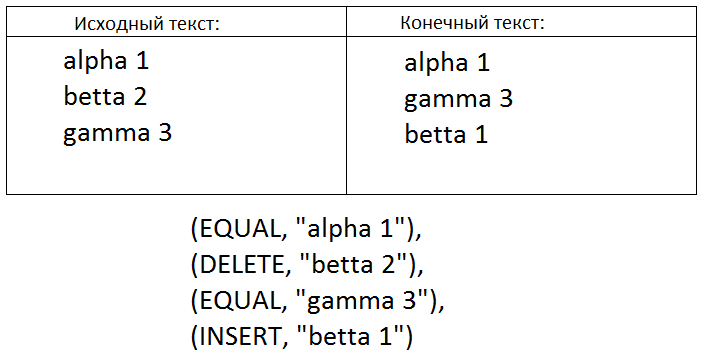
\includegraphics[scale=0.9]{diffResult.png}
\caption{\emph{Пример результата работы diff алгоритма}}
\label{pr:image5}
\end{center}
\end{figure}

\subsubsection{Алгоритм}

Исходный документ преобразуется в DOM дерево, и из него извлекаются все выделенные фрагменты требований, которые нужно перенести. Затем осуществляется преобразование исходного и конечного документа в текстовые данные без XHTML разметки, при этом позиции в исходном тексте извлеченных ранее фрагментов требований запоминаются. Два полученных текста подаются на вход Diff алгоритму, который возвращает список операций, описывающих разницу между исходным и конечным документом.

После окончания работы Diff алгоритма для каждого фрагмента требования из исходного текста определяется, находился ли он в блоке EQUAL результата работа Diff, и если да, то осуществляется перенос соответствующих тегов требования в DOM дерево конечного документа. В противном случае считается, что фрагмент перенести не удалось. Обновленный конечный документ восстанавливается по измененному DOM дереву.

Таким образом, алгоритм можно представить в виде диаграммы, изображенной на рисунке \ref{pr:image6}.

\begin{figure}[h]
\begin{center}
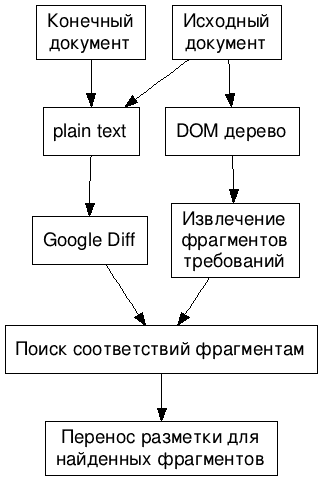
\includegraphics[scale=0.7]{reqSolutionPresentation.png}
\caption{\emph{Диаграмма алгоритма переноса разметки требований системы Requality}}
\label{pr:image6}
\end{center}
\end{figure}

\subsubsection{Характеристики алгоритма, реализованного в Requality}

Важной особенностью такого подхода к решению задачи является независимость получения результата от разницы между разметкой исходного и конечного документов. Если в новой версии документа была использована разметка, отличная от старого, то это не повлияет на эффективность работы алгоритма, поскольку разметка документов используется только при поиске фрагментов требований. С другой стороны, решение, основанное на использовании diff-алгоритма, перестает работать в случае перестановки разделов в конечном документе, и может работать существенно хуже в случае добавления большого количества новых разделов и текста.

Помимо этого, в текущей реализации этого алгоритма есть фрагменты, соответствие которым находится, однако перенос не осуществляется в связи с различными трудностями работы с DOM моделью документа.

\subsection{Предлагаемое решение}

Основной идеей решения поставленной задачи, которое описывается в данной работе, является локализация места конечного документа, в котором осуществляется поиск соответствия фрагменту, выделенному в исходном документе. В качестве места, в котором нужно осуществлять поиск, в конечном документе выбирается подраздел, соответствующий (в дальнейшем будет описано, как) подразделу исходного документа, содержащего искомый фрагмент требования.

После проведения этой операции размер текста, в котором нужно найти соответствие фрагменту требования, считается достаточно маленьким для применения алгоритма прямого поиска. В том случае, если совпадение с текстом фрагмента было найдено, осуществляется перенос разметки в соответствующее место конечного документа.

\subsection{Внутреннее представление документа}

Однако DOM дерево, полученное из исходного и конечного документов, не удовлетворяет полностью потребностям такого решения - текст раздела в таком дереве не привязан к заголовку, а заголовки, являющиеся вложенными в документе, в DOM дереве находятся на одном уровне иерархии. Таким образом, DOM модель не отражает структурную разметку документа.

Поэтому для удобства работы с иерархией разделов документов было решено осуществлять построение на основе DOM моделей документов деревья, позволяющие проще отслеживать вложенность разделов и связь текстов разделов с их заголовками.

Пример DOM дерева документа, и построенного по нему дерева структурной разметки можно наблюдать на рисунках \ref{ris:DOMtree} и \ref{ris:MYtree} соответственно:

\begin{figure}[h]
\begin{center}
\begin{minipage}[h]{0.55\linewidth}
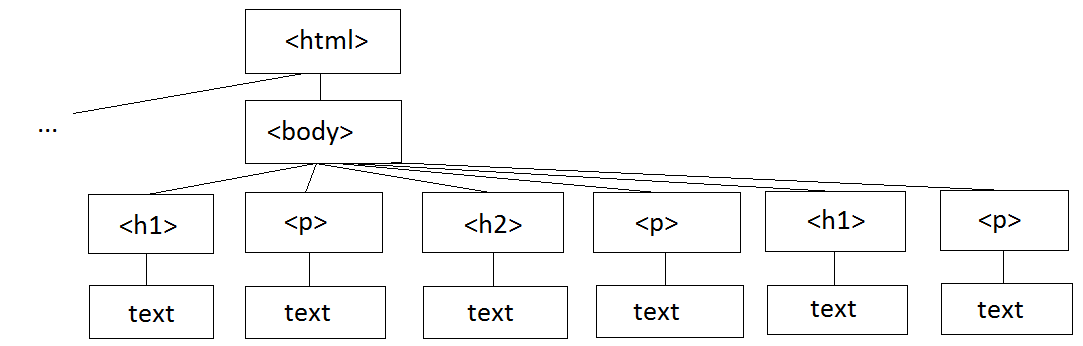
\includegraphics[width=1\linewidth]{good_dom_tree.png}
\caption{\emph{DOM дерево документа.}} %% подпись к рисунку
\label{ris:DOMtree} %% метка рисунка для ссылки на него
\end{minipage}
\hfill 
\begin{minipage}[h]{0.4\linewidth}
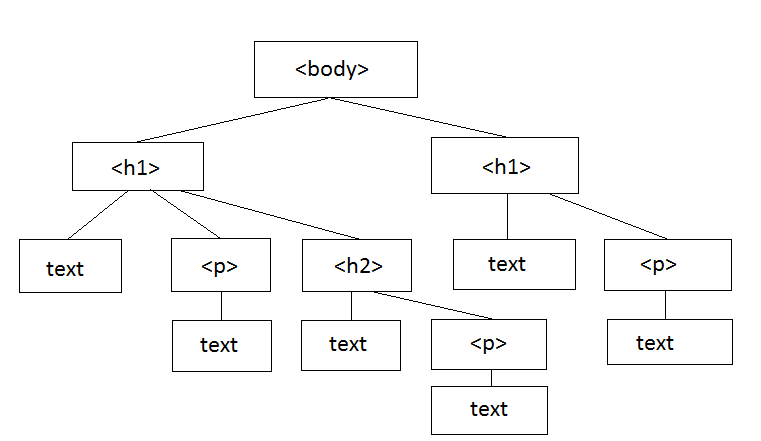
\includegraphics[width=1\linewidth]{my_tree}
\caption{\emph{Построенное дерево структурной разметки.}}
\label{ris:MYtree}
\end{minipage}
\end{center}
\end{figure}

Основываясь на введенном новом представлении документа, определим следующие понятия:

\textbf{Путь до раздела документа} – список вершин в пути в дереве разметки документа до вершины, соответствующей разделу.

\textbf{Путь до фрагмента требования} – путь до вершины дерева разметки максимальной глубины, соответствующей разделу, в котором содержится этот фрагмент.

\subsection{Алгоритм}

Таким образом, алгоритм переноса разметки требований между версиями документа выглядит следующим образом:

\begin{enumerate}
\item Извлечь содержимое исходного и конечного документов при помощи JDOM

\item Построить на основе DOM деревьев документов деревья структурной разметки

\item Извлечь требования из дерева исходного документа

\item Для каждого объединения фрагментов требования:

\begin{enumerate}

\item Получить путь до объединения фрагментов требования

\item Получить по дереву разметки конечного документа путь до соответствующего раздела

\item Найти вхождение текста объединения фрагментов в полученном разделе.

\item Если путь в дереве разметки конечного документа или вхождение текста объединения фрагментов в разделе конечного документа не было найдено, считать, что перенос каждого фрагмента из объединения осуществить не удалось. В противном случае - изменить структуру части дерева разметки, соответствующей разделу конечного документа, добавив в неё фрагменты требования

\item Изменить структуру соответствующей разделу части DOM дерева конечного документа

\end{enumerate}

\item Изменить конечный документ в соответствии с изменением структуры его DOM дерева

\end{enumerate}

\subsection{Характеристики предложенного алгоритма}

В силу особенности построения дерева разметки для исходного и конечного документов, добавление, изменение или удаление разделов, не содержащих фрагментов требований, не влияет на эффективность работы алгоритма. Помимо этого, перестановка разделов в конечном документе так же не влияет на перенос фрагментов. 

Однако изменения заголовков разделов, по которым локализуется место поиска соответствия объединению фрагментов требования, а так же изменения вложенности подразделов, в которых ищутся фрагменты, влияют на перенос разметки в конечный документ - если полное соответствие пути до объединения фрагментов в дереве разметки исходного документа не было найдено, перенос фрагментов не осуществляется.

Помимо этого стоит отметить, что предложенный алгоритм гораздо проще обобщить на случай, когда в конечном документе существует лишь частичное соответствие тексту объединения фрагментов, чем алгоритм, основанный на применении diff. Подробнее об этом будет рассказано в заключении.